\chapter{Nuclear Data}

\fancyhead[L]{University of Surrey, November 2026 \hfill Professor David Jenkins}
\label{nucdat}
\section{Introduction}
The following notes are based on \textit{Nuclear Data: A Primer} by Jenkins and Wood in preparation for the PLANET baseline training lectures in nuclear structure. Additional primary references: 
\begin{itemize}
    \item Krane: \textit{Introductory Nuclear Physics}
    \item Bertulani: \textit{Nuclear Physics in a Nutshell}
    \item Choppin, Rydberg, Liljenzin and Ekberg: \textit{Radiochemistry and Nuclear Chemistry} 4ed
    \item Wong\label{Wong}: \textit{Introductory Nuclear Physics} 2ed
    \item Casten: \textit{Nuclear Structure from a Simple Perspective}
    \item Heyde: \textit{Basic Ideas and Concepts in Nuclear Physics} 3ed
    \item Loveland, Morrissey, Seaborg: \textit{Modern Nuclear Chemistry} 2ed
    \item Rohlf: \textit{Modern Physics from \(\alpha\) to \(Z^0\)}. Chapters \(9\) - \(11\)
    \item Shultis, Faw: \textit{Fundamentals of Nuclear Science and Engineering}
    \item Andreyev: \textit{Third Year Nuclear II Lecture Notes}
    \item Wilson-Rae/Cavill: \textit{Fourth Year Quantum V Lecture Notes}
\end{itemize}


\section{Nuclear Data Sets}
Nuclear data are mostly organised by mass chains or \(A\) chains i.e. data is evaluated for nuclear isobars (sometimes an \(A\) chain will contain a single isotope). Recall that there are various categories of isotopes - groups of nuclei that share a common property:
\begin{itemize}
    \item Isobar: Same mass, \(A = N + Z\).
    \item Isotope: Same proton number, \(Z\).
    \item Isotone: Same neutron number, \(N\).
    \item Isomer: Same mass and proton number, but with some nucleons in an excited state e.g. metastable Technetium-99, \ce{^{99m}Tc}.
\end{itemize}
Instead of \(A\) chains, groups occassionally produce `horizontal' compilations and evaluations i.e. a compilation or evaluation of a specific nuclear property across an entire range of \textit{A}, \textit{Z} and \textit{N} - referred to as a mass surface. An example of a horizontal compilation is that of nuclear masses, maintained by the Atomic Mass Evaluation (AME) network. 
Examples of commonly used nuclear databases:
\begin{itemize}
    \item Evaluated Nuclear Structure Data File (\ensdf) and Experimental Unevaluated Nuclear Data List (\xundl) maintained by the National Nuclear Data Centre (NNDC). It also publishes evaluations by \(A\) chain in the journal \href{https://www.sciencedirect.com/journal/nuclear-data-sheets}{\textit{Nuclear Data Sheets}} and has an interactive plotting tool, \href{https://www.nndc.bnl.gov/nudat3/}{NuDat3}.
    \item Specialised evaluations appear in journals such as \href{https://www.sciencedirect.com/journal/atomic-data-and-nuclear-data-tables}{\textit{Atomic Data and Nuclear Tables}} and \href{https://iopscience.iop.org/journal/1674-1137}{\textit{Chinese Physics C}}. Review articles on special topics appear in \href{https://www.sciencedirect.com/journal/physics-reports}{\textit{Physics Reports}}, \href{https://www.sciencedirect.com/journal/progress-in-particle-and-nuclear-physics}{\textit{Progress in Particle and Nuclear Physics}}, \href{https://iopscience.iop.org/journal/0034-4885}{\textit{Reports on Progress in Physics}} and \href{https://journals.aps.org/rmp/}{\textit{Reviews of Modern Physics}}.
\end{itemize}

\section{Gross Properties of Nuclei}
Gross properties are those which involve the entire nucleus - radius and mass fall within this definition. 

\subsection{Measuring Radii}
A nucleus doesn't have a sharp surface - it is diffuse. This is deduced from inferring charge density distributions, \(\rho(r)\), using elastic electron scattering. Charge density as a function of the distance from the centre of the nucleus obeys a typical Fermi distribution.

\[\rho (r) = \frac{\rho_0}{1+e^{r-\frac{R_{1/2}}{a}}}\]

Where \(\rho (R_{1/2})=\frac{1}{2}\rho_0\) and \(a\) gives the width of the surface diffuseness. The width of the interval where density decreases from 90\% of \(\rho_0\) to 10\% of \(\rho_0\) is \(4.4a\). These diffuse effects are mainly due to p-n interactions. Nucleon density is approximately constant inside the nucleus. For most nuclei, there are more neutrons than protons so the individual density distributions would both follow the same shape of a Fermi distribution, but the proton curve would be lower. 

Instead of electron scattering, x-ray spectroscopy be used on muonic atoms to provide further information on the density distribution. With their increased mass, muons exist closer to the nucleus than electrons so a higher fidelity is possible.

\subsubsection*{RMS Charge Radius and Isotope Shifts}
Since nuclear surface diffuseness is not a fixed geometric property, it is convenient to define an rms charge radius, \(\langle r^2 \rangle ^{1/2}\), for a given nuclear species (a given \(Z\) and \(N\)). This is a well-defined quantity and is unique for each nuclear species. These data are usually plotted as isotope shifts - small variations in charge radius along isotopic chains (measured using optical hyperfine spectroscopy), between a given nucleus and a specified isotope of that nucleus i.e. they are plotted for a fixed \(Z\) as a function of \(N\).

When \(\langle r^2 \rangle ^{1/2}\) values are plotted as a function of \(A\), they follow the liquid drop model closely. Following:
\[\left[\frac{5}{3}\langle r^2\rangle\right]^{1/2}=R_0 A^{1/3}\]

\begin{figure}[H]
\captionsetup{width=.75\textwidth}
    \centering
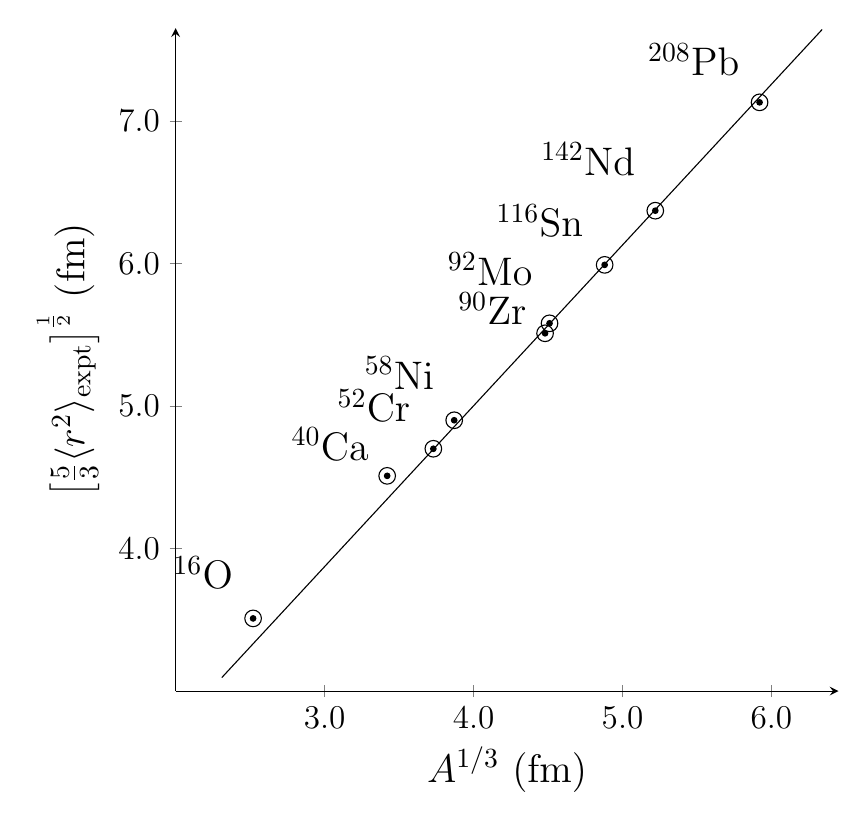
\begin{tikzpicture}
\begin{axis}[
    width=10cm, height=10cm,
    axis lines=left,
    xmin=2, xmax=6.45,
    ymin=3, ymax=7.65,
    xtick={3.0,4.0,5.0,6.0},
    ytick={4.0,5.0,6.0,7.0},
    yticklabel style={/pgf/number format/fixed, /pgf/number format/fixed zerofill, /pgf/number format/precision=1},
    xticklabel style={/pgf/number format/fixed, /pgf/number format/fixed zerofill, /pgf/number format/precision=1},
    xlabel={$A^{1/3}$ (fm)},
    ylabel={$\left[\frac{5}{3}\langle r^2\rangle_{\mathrm{expt}}\right]^{\frac{1}{2}}$ (fm)},
    xlabel style={font=\Large},
    ylabel style={font=\Large},
    tick label style={font=\large},
    clip=false,
]

% Straight-line guide
\addplot[black, thin, domain=2.31:6.34] {1.128*(x-2.31)+3.095};

% Data points (circled dots)
\addplot[only marks, mark=*, mark size=1pt] coordinates {
    (2.52,3.51) (3.42,4.51) (3.73,4.70) (3.87,4.90)
    (4.48,5.51) (4.51,5.58) (4.88,5.99) (5.22,6.37) (5.92,7.13)
};
\addplot[only marks, mark=o, mark size=3pt] coordinates {
    (2.52,3.51) (3.42,4.51) (3.73,4.70) (3.87,4.90)
    (4.48,5.51) (4.51,5.58) (4.88,5.99) (5.22,6.37) (5.92,7.13)
};

% Nuclide labels
\node[anchor=south east, font=\Large] at (axis cs:2.45,3.65) {$^{16}$O};
\node[anchor=south east, font=\Large] at (axis cs:3.36,4.55) {$^{40}$Ca};
\node[anchor=south east, font=\Large] at (axis cs:3.64,4.82) {$^{52}$Cr};
\node[anchor=south east, font=\Large] at (axis cs:3.80,5.05) {$^{58}$Ni};
\node[anchor=south east, font=\Large] at (axis cs:4.42,5.50) {$^{90}$Zr};
\node[anchor=south east, font=\Large] at (axis cs:4.46,5.78) {$^{92}$Mo};
\node[anchor=south east, font=\Large] at (axis cs:4.80,6.12) {$^{116}$Sn};
\node[anchor=south east, font=\Large] at (axis cs:5.15,6.55) {$^{142}$Nd};
\node[anchor=south east, font=\Large] at (axis cs:5.85,7.25) {$^{208}$Pb};

\end{axis}
\end{tikzpicture}
    \caption{Nuclear rms charge radii compared to the liquid drop model. 
    Almost exact for \(A\geq90\), deviation for \(A < 90\) due to surface 
    diffuseness. Adapted from fig. 1.7 in \textit{Primer} \anth}
    \label{rms_vs_A}
\end{figure}



Figure \ref{rms_vs_A} shows that nuclear size scales with \(A\). If the nuclear binding force were long ranged and attractive, the size of a nucleus would shrink with a larger number of nucleons due to the increased binding. This is what happens for atoms, due to the long ranged Coulomb attraction between the \(+Ze\) charge of the nucleus and the electrons. 

\subsection{Measuring Masses}
Masses are usually measured for atoms, whereas radii are measured for nuclei. Atoms are easier to handle than nuclei, producing a bare nucleus would involve stripping away all electrons leaving a highly charged ion which would be neutralised by capturing electrons from its environment. Instead, singly charged ions are used because they are easy to maintain and manipulate under a vacuum with E and B fields. 

\subsubsection*{Nuclear vs Atomic Binding Energy}
The mass of a nucleus is less than the mass of its constituent parts due to binding energy. Binding energy is on the order of 1\% the mass of the total nucleus. For an atom, masses also include the mass of the electrons minus the electronic binding energy. However, electronic binding energy is comparatively very small, less than the measurement uncertainty of the total atomic mass (note that this does not mean atomic binding energy is unknowable, it can be inferred by summing ionisation potentials for successive removal of the electrons in a given atom). Hence, we only consider nuclear binding energy, \(B(Z, N)\).

\[M(Z, N) = Zm_p + Nm_n + Zm_e - B(Z, N)\]

\subsubsection*{Binding Energy per Nucleon}
Binding energy alone, when plotted against \(A\) is monotonic. However, plotting binding energy per nucleon, \(B/A\), we make the following observations. 
\begin{enumerate}
    \item The vast majority of nuclei, \(20 < A < 200\) have an almost constant binding energy per nucleon, \(8.3 \pm 5\%\) MeV/nucleon.
    \item Maximum \(B/A\) occurs at \ce{^{62}Ni}.
    \item There is a steep decline in \(B/A\) down to the lightest nuclei.
    \item There is a steady and slowly steepening decline in \(B/A\) toward heavy nuclei.
\end{enumerate}
We can make the following interpretations of the above observations.
\begin{enumerate}
    \item \textbf{Constancy of B/A Beyond \ce{^{62}Ni}}: The force binding nucleons must be short ranged as it will mostly only influence its nearest neighbours, resulting in a saturation of the binding i.e. there can only be so many neighbours of a given nucleon. This is analogous to water having a constant boiling point (\(L_v\)) at STP, no matter the amount of water being heated. If the binding force were long ranged and attractive, binding energy would be non-linear and increasing. 
    \item \textbf{Maximum Value of B/A}: A result of the balance between the minimum surface-area-to-volume ratio and the minimum Coulomb repulsion between protons. The occurence at \ce{^{62}Ni} is coincidentally near where stellar fusion stops, but it does not mark a profound nuclear property. 
    \item \textbf{Steep Decline in B/A for Light Nuclei}: Also a consequence of the short range of the strong nuclear force. In light nuclei, almost all nucleons are at the surface, hence they do not have a full set of neighbours as most nucleons do in a heavy nucleus. So, the binding energy of a light nucleus is unsaturated.
    \item \textbf{Slow Decline in B/A for Heavy Nuclei}: A long ranged and repulsive force would result in binding energy being non-linear and decreasing - seen in heavy nuclei because of the increasing number of protons and their long ranged Coulomb repulsion.
\end{enumerate}

\input{exercises/1-4_binding_energy}

\input{exercises/1-7_uranium_fission}

\input{exercises/1-11_electronic_binding_2H}



\newpage
\subsection{Differences in Radii and Masses}
\subsubsection{Neutron Separation Energies}
By plotting differences in gross properties, shell structure becomes apparent. Figure \ref{isotopicshift} shows marked increase in isotope shifts at magic numbers.

\begin{figure}[H]
    \centering
    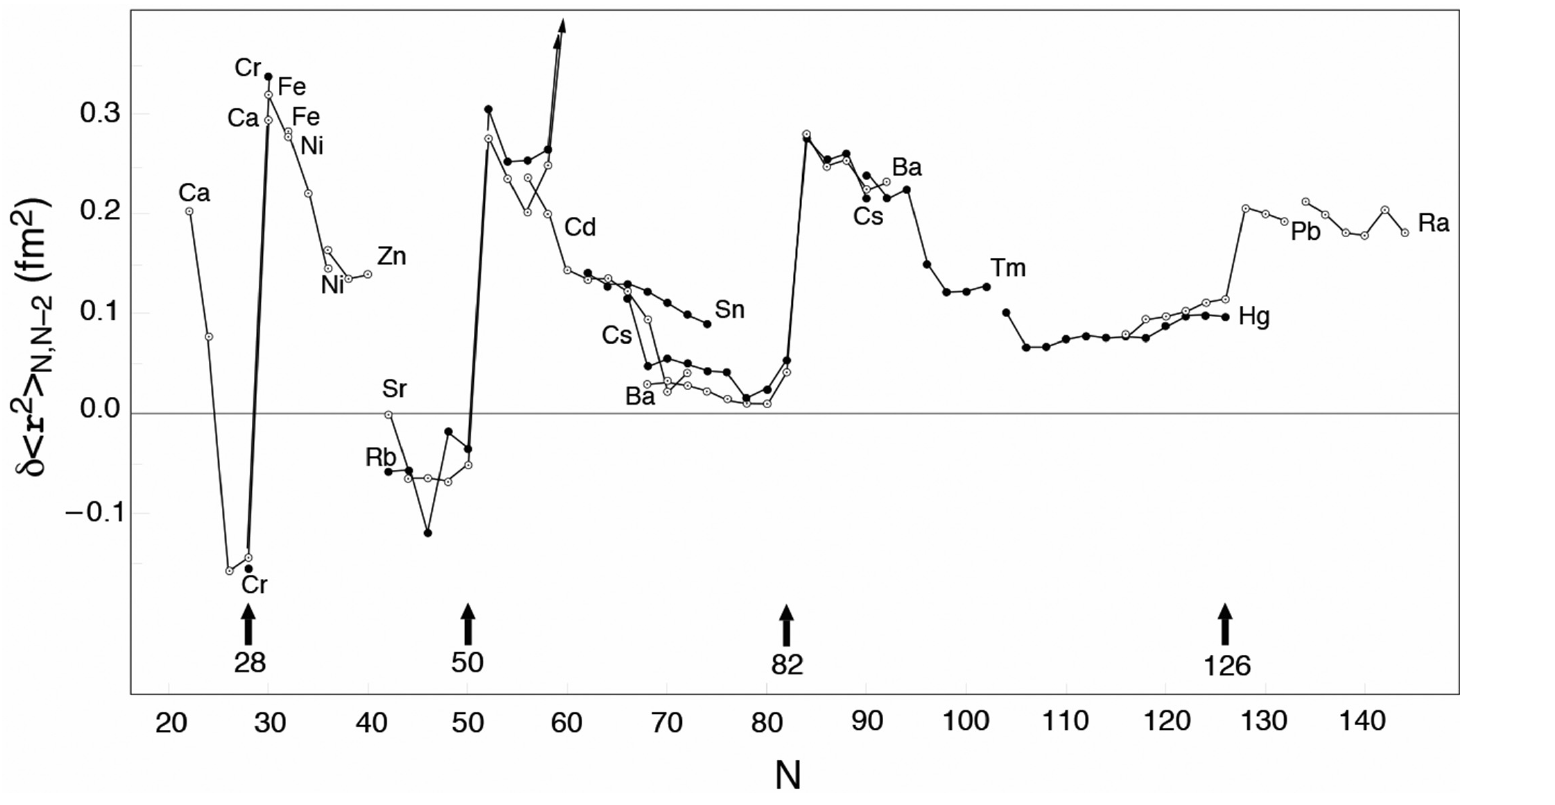
\includegraphics[width=0.8\textwidth]{assets/2.1.1_isotope_shifts.png}
    \caption{Isotope shifts for specific isotopic sequences of nuclei. Fig. 1-9 of \textit{Primer}.}
    \label{isotopicshift}
\end{figure}

Differences in binding energies are termed separation energies. One-neutron separation energy is defined as:
\[S_n = -M(A,Z,N) + M(A-1,Z,N-1)+m_n\]

Observations to note from figure \ref{Sn}:
\begin{enumerate}
    \item Odd-even staggering of \(S_n\).
    \item Discontinuities, `steps' down, with increasing \(N\) or \(A\).
    \item Between the steps, the trend is smooth and down-sloping with increasing \(N\) or \(A\).
\end{enumerate}

\begin{figure}[H]
    \centering
    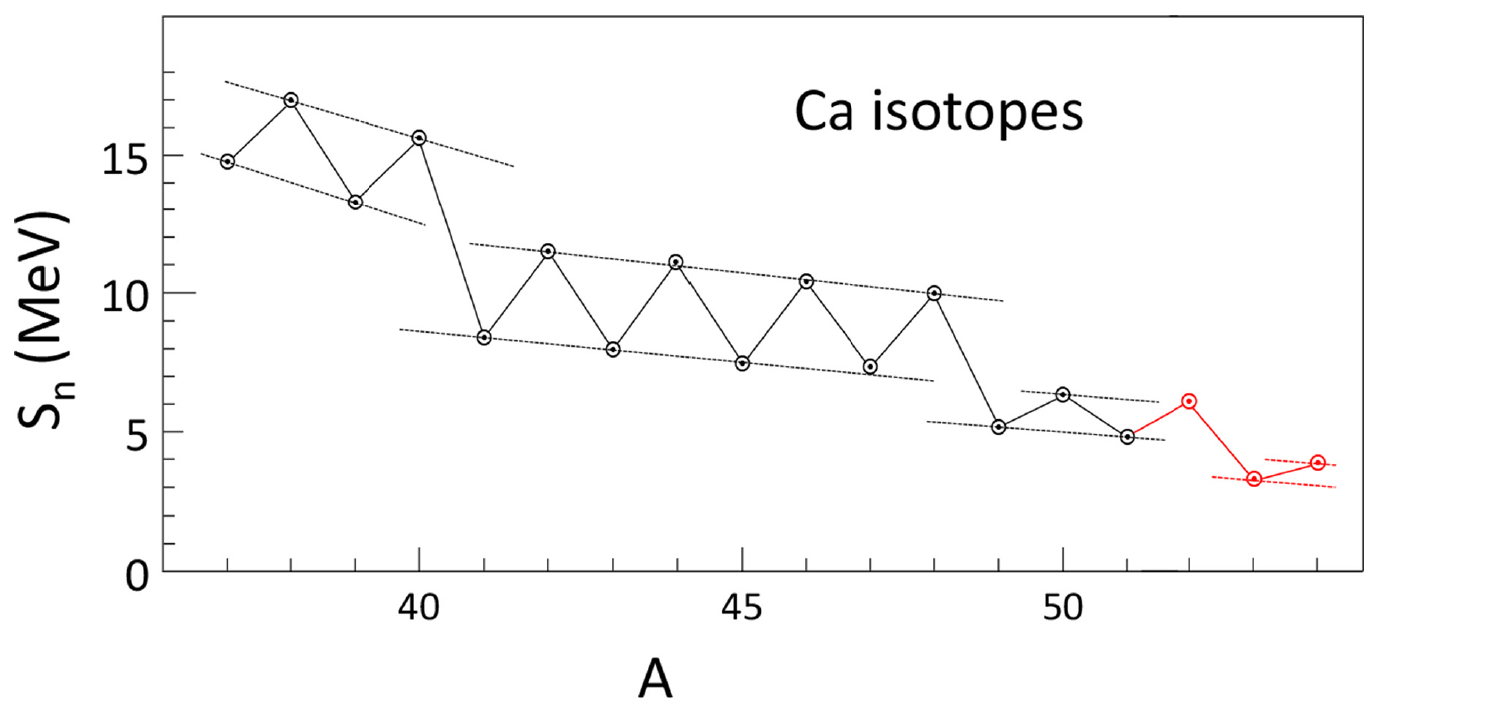
\includegraphics[width=\linewidth]{assets/2.1.1_Sn.png}
    \caption{One-neutron separation energies. Data from \href{https://amdc.impcas.ac.cn/}{\ul{AMDC}} files. Fig. 1.10 \textit{Primer}. The red points represent new data, measured within recent years.}
    \label{Sn}
\end{figure}


We can make the following interpretations of the above observations.
\begin{enumerate}
    \item \textbf{Odd-even Staggering}: Due to enhanced binding when the neutron number is even. Similarly observed for \(S_p\). An effect termed pairing. Manifestation of quantum mechanical correlations.
    \item \textbf{Steps Down}: Due to `shell closures'. From left to right in the figure, successive neutrons are removed. Nucleons are confined in an average potential generated by all of the other nucleons. Nucleons sequentially fill orbitals. When an energy gap is reached in the removal process, there is a sudden step up in the removal energy. This effect is more clearly seen for two-neutron separation energies, figure \ref{S2n}.
    \item \textbf{Sloping Down Between Steps}: Due to the confining potential changing with \(\sim A^{1/3}\). As \(A\) increases, potential width increases and the potential becomes shallower.
    \item \textbf{Shell Closure Locations}: Only occur at the classical magic numbers, 20, 28, 50, 82, 126.
\end{enumerate}

\begin{figure}[H]
    \centering
    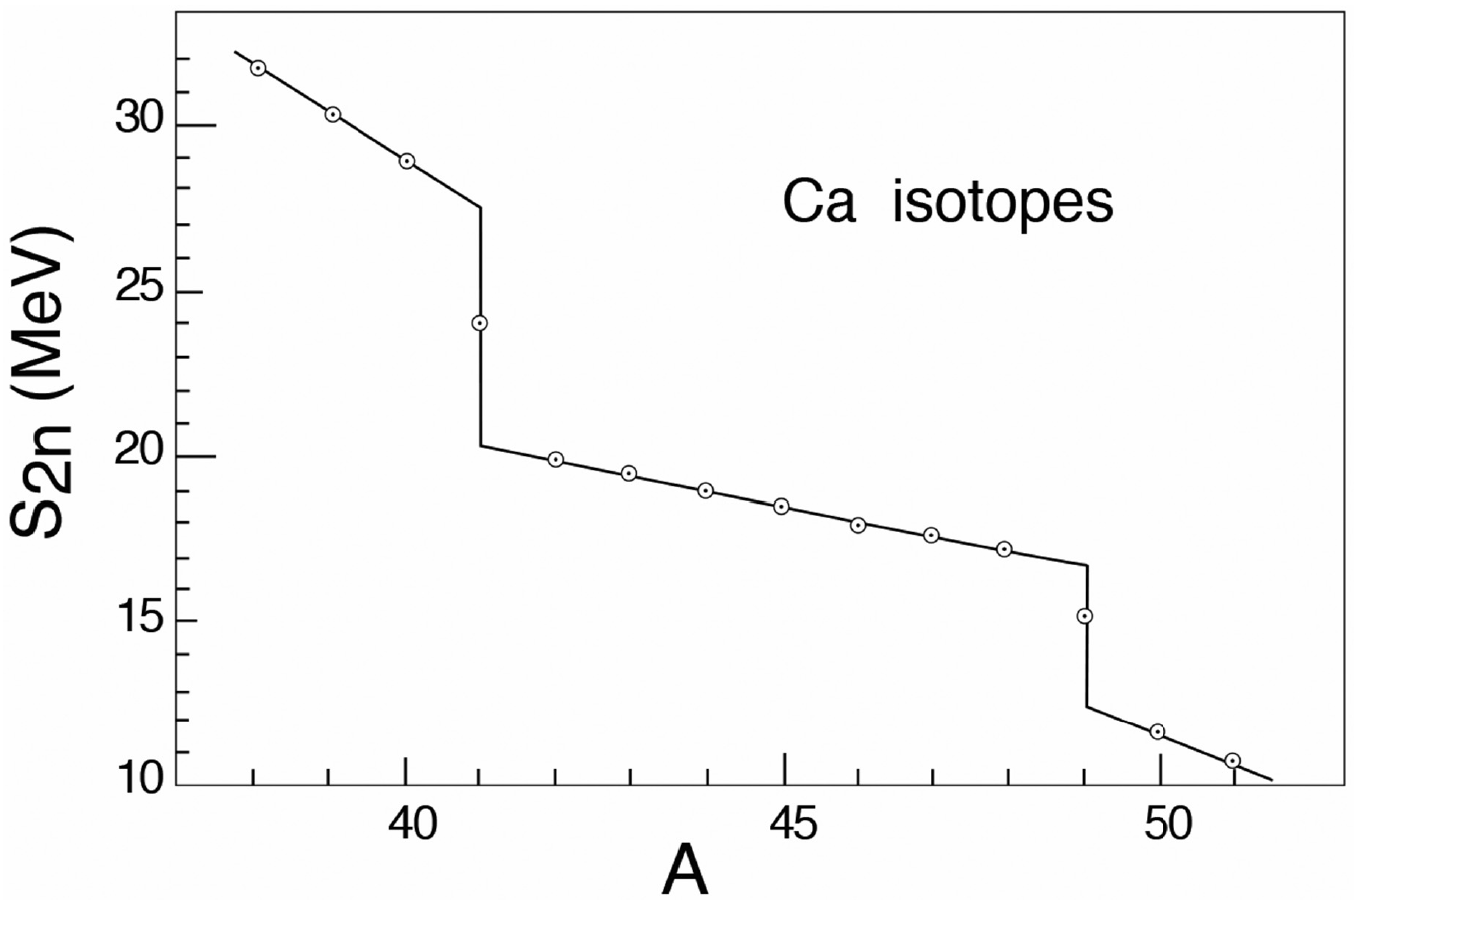
\includegraphics[width=\linewidth]{assets/2.1.1_S2n.png}
    \caption{Two-neutron separation energies. Data from \href{https://amdc.impcas.ac.cn/}{\ul{AMDC}} files. Fig. 1.11 \textit{Primer}.}
    \label{S2n}
\end{figure}

\subsubsection{Nuclear Shell Model}
The shell structure of nuclei was the first major step in organising nuclear data using quantum mechanics. It was formalised in 1949. The shell structure led to the nuclear shell model. 

It is natural to suppose that nuclei are always spherical, in order to minimise the surface area and thus maximise the binding energy (by way of saturating the short ranged intra-nucleon force). However, by measuring quadrupole moments, it is known that most nuclei are deformed. Note that the first evidence for nuclear deformation came from optical hyperfine spectroscopy conducted by Sch\"{u}ler and Schmidt and interpreted by Casimir in the mid-1930s. Prolate (rugby ball shaped) nuclei far outnumber oblate (frisbee shaped) nuclei. It is currently unknown as to why this occurs. Note that in figure \ref{quadrupole}, closed shell nucleon numbers are consistent with zero deformation. 

\begin{figure}[H]
    \centering
    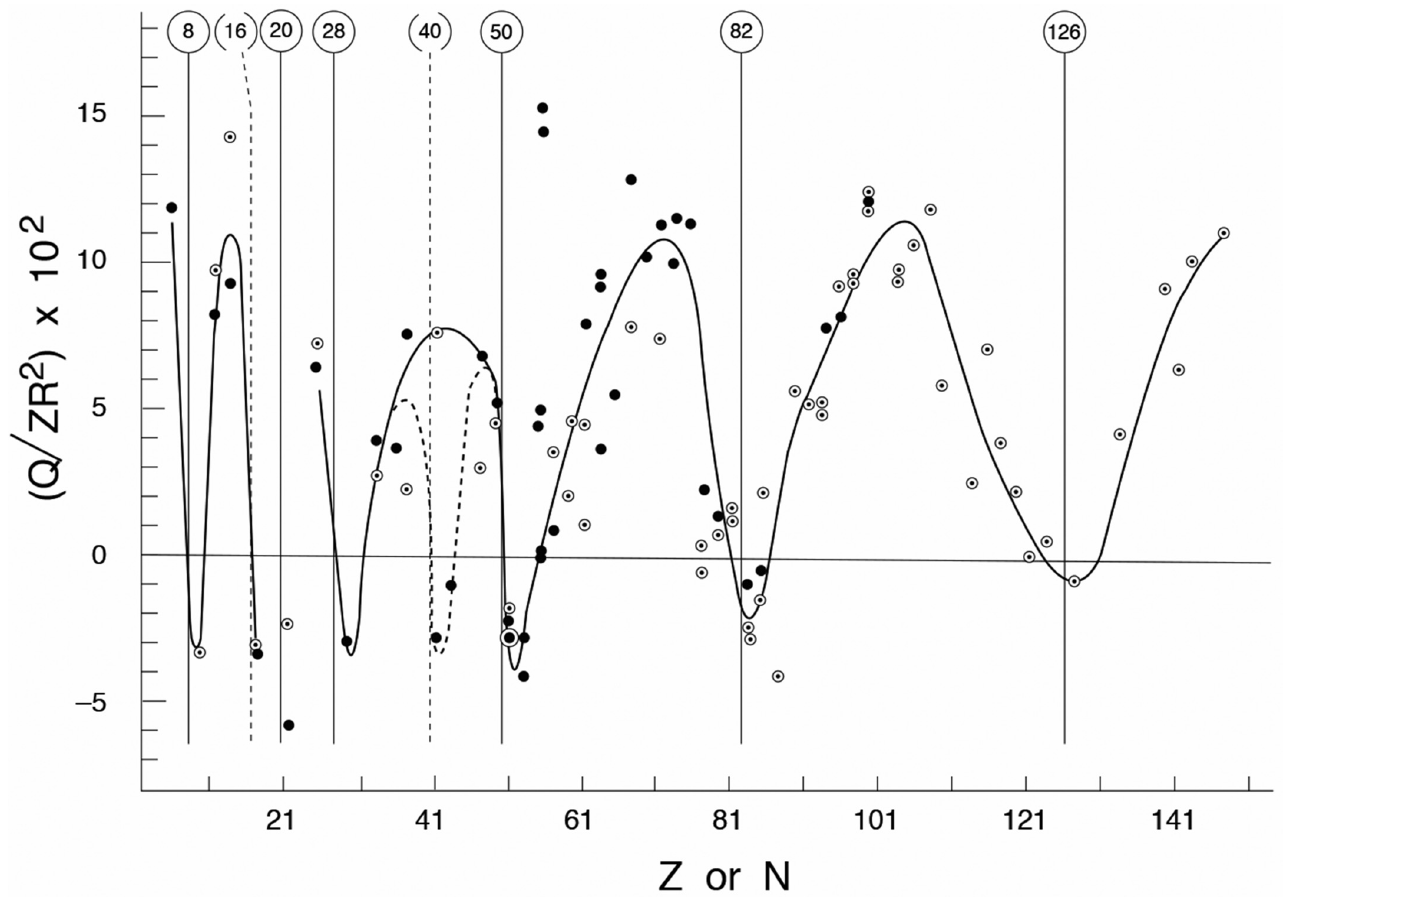
\includegraphics[width=\linewidth]{assets/2.1.1_quadrupole.png}
    \caption{Normalised electric quadrupole moments. Positive values indicate prolate shapes, negative values indicate oblate shapes. \textit{Primer} Fig. 1.14.}
    \label{quadrupole}
\end{figure}

There are limits to the existence of nuclei w.r.t. the possible combinations of \(Z\) and \(N\) that survive long enough to be isolated for study in a laboratory. Proton and neutron `drip lines' are the borders beyond which nuclei do not exhibit bound states. Outside these borders, trying to add another nucleon just causes it to fall off. The neutron drip line has very limited information compared to the proton drip line. This is due to the conditions needed to produce the neutron-rich nuclei, present in astrophysical processes e.g. the R-process. In such environments (perhaps neutron stars), these nuclei may have a fleeting existence, sufficient for the species to undergo a nuclear reaction. The most consequential example would be the existence of \ce{^8Be} which exists long enough in massive stars to lead to the formation of carbon, \ce{^8Be + ^4He \rightarrow ^{12}C}. 

\subsubsection{Beta Decay and Mass Parabolas}
Along a set of isobars (i.e. for a given value of \(A\)), plotting mass excess as a function of \(Z\) reveals that there is a parabolic behaviour. 

\begin{figure}[H]
    \centering
    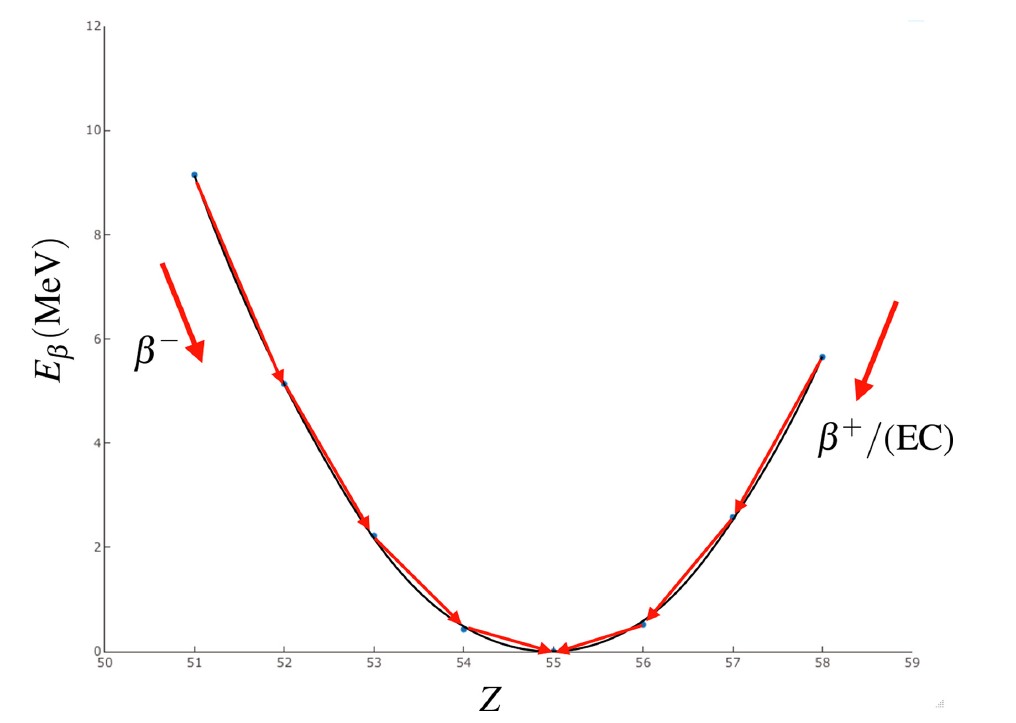
\includegraphics[width=0.8\textwidth]{assets/2.1.1_beta1.png}
    \caption{The \(A=133\) mass parabola. The stable isotope is \ce{^{133}_{55}Cs}, the energies are set relative to this and plotted as energies available for beta decay. Note that the decay energy for \ce{^{133}Ba \rightarrow ^{133}Cs} is \(517\) keV, less than the \(1022\) keV needed for beta plus decay, so it can only occur via electron capture. \textit{Primer} Fig. 1.16}
    \label{beta1}
\end{figure}

These parabolas join up to produce the line of stability on the chart of nuclides. The minimum of a given parabola is the most stable \(Z\) for the given \(A\), suggesting that the isobars decay towards this minimum via processes where \(A\) is constant: beta decay. Nuclei on the left side of the parabola (lower \(Z\)) undergo \(\beta ^-\) decay and nuclei on the right undergo \(\beta ^+\) decay. A competing process to \(\beta ^+\) decay is electron capture, where a bound atomic electron is subsumed into the nucleus by a proton, producing a neutron and releasing an electron neutrino (plus some x-rays, from electrons de-exciting to fill the K shell vacancy left by the electron). This is a much lower energy process than \(\beta ^+\) decay, which requires at least \(1.02\) MeV - twice the mass of an electron - to create the positron. Electron capture is more likely in heavier elements, where higher energies are less likely and electrons exist closer to the nucleus. 
There is also a possibility for certain even-even nuclei to undergo double beta decay. 

\begin{figure}[H]
    \centering
    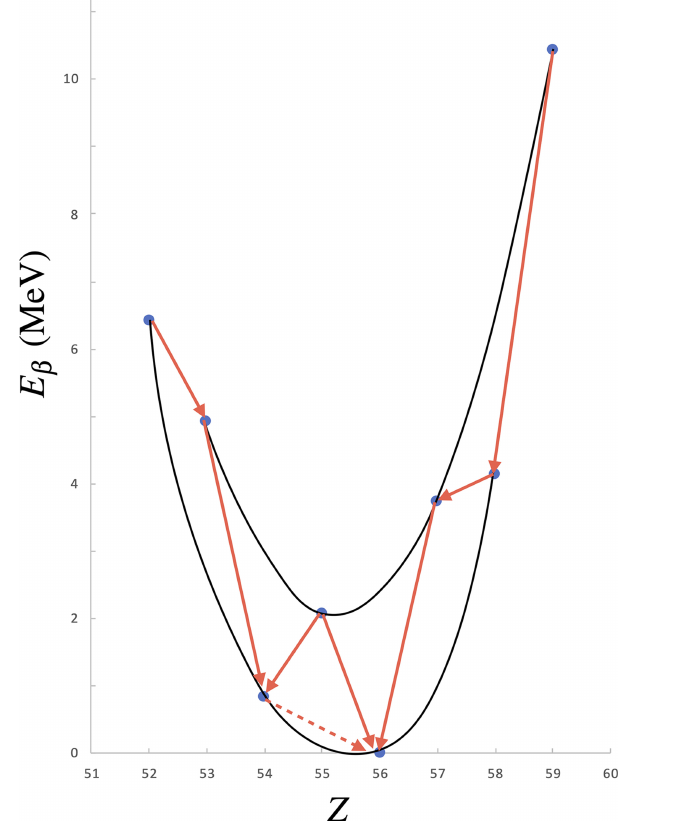
\includegraphics[width=0.7\textwidth]{assets/2.1.1_beta2.png}
    \caption{The \(A=134\) mass parabolas. Two parabolas exist for even-\(A\) nuclei due to the attractive pairing term in the SEMF. So, \ce{^{134}_{55}Cs \rightarrow ^{134}_{54}Xe} by beta plus and \ce{^{134}_{55}Ca \rightarrow ^{134}_{56}Ba} by beta minus. The dashed arrow represents a double beta decay, the half life for this process is \(>10^{18}\) y and has yet to be studied for \ce{^{134}Xe}. \textit{Primer} Fig. 1.17.}
    \label{beta2}
\end{figure}

\input{exercises/1-13_mass_parabolas_stability_line}

\input{exercises/1-14_SEMF_exploration}

\subsection{Alternative Decay Processes to Beta Decay}
Nuclear masses reveal another property of nuclei that is usually hidden: a variety of processes besides beta decay are energetically favourable. For example, alpha decay, proton decay and emission of heavy nuclear clusters such as \ce{^{14}C}. The alpha particle is the most strongly bound nuclear system - evident because it occurs much more frequently than emission of single protons and neutrons. These processes are fairly rare and only occur near the driplines, whereas alpha decay occurs for a whole host of heavy nuclei. 

Alpha decay from a nucleus (\(A, Z, N\)) is energetically favourable if the following mass relation holds.
\[M(A, Z, N) > M(A-4, Z-2, N-2) + M(\ce{^4He})\]
In order for this to happen, the alpha particle must tunnel through a Coulomb barrier. Such barriers exist for all charged-particle decay processes are nuclei. For many nuclei, these processes are energetically favourable but are too improbable (small reaction cross-section) for observation. This is usually due to:
\begin{itemize}
    \item A poor overlap of the initial and final state wavefunctions: the initial states look nothing like the final bound state.
    \item Competing decay channels: e.g. if the cross-section for fission is much lower than the scattering cross-section then fission will be practically never observed, even if it releases a greater amount of energy.
    \item Suppression by the weak force: If a reaction involves a proton turning into a neutron, it is governed by the weak force. When comparing the weak and strong force cross-sections at the same energy, the weak could be of the order \(10^{20}\) times weaker than the cross-section of the strong. This is the reason why we cannot easily recreate the proton-proton chain on Earth, its cross-section is too small for laboratory detection.
\end{itemize}

\input{exercises/1-6_solar_energy}

\subsection{Superheavy Elements and the Periodic Table}
The superheavy elements represent the one direction in which combinations of \(Z\) and \(N\) are still being explored with no known limitations, except the difficulty of making them in the laboratory. Currently the farthest reach is element \(118\), Oganesson (in the form of \ce{^{294}_{118}Og^{176}}), achieved by bombarding a \ce{^{149}Cf} target with a beam of \ce{^{48}Ca} nuclei with the `evaporation' of three neutrons. It is believed to be a continuation of the noble gases, hence the name ending -on (...krypton, xenon, radon).

Implicit in nuclear physics is Mendeleyev's periodic table of chemical elements. It can be conjectured that the limit of the periodic table will be determined by Coulomb repulsion of protons and the increasing likelihood of near instant spontaneous fission. The half life of an isotope at such a limti will bedictated by the Coulomb barrier, through which the separating pair of fission fragments must tunnel. Thus, the most promising direction for synthesising new superheavy elements would be to find a way to `add' more neutrons. 

The organisation of the chemical elements reflects the electron shell structure, this also mainfests in the atomic ionisation potentials (electron `separation' energies). Shell structure in atoms and in nuclei reflect the same underlying quantum mechanics: many-body systems behave as a collection of independent particles confined by an average single-particle potential. While nuclei exhibit correlations (manifestly, not independent particle behaviour), independent particle behaviour was the primary insight into nuclear structure that launched the quantum mechanical description of nuclei.

For a concise perspective on how science has developed its understanding of the nucleus, see an article written by Bethe in 1999 for the journal \textit{Reviews of Modern Physics}, reproduced in \hyperref[bethe]{the appendix}.



\subsection{Nuclear Reaction Notation}
See \ref{Wong} page 16. The usual type of final state in a reaction is two body i.e. a projectile, \(a\), is incident upon a target particle, \(A\), from which a particle, \(b\) is scattered away, leaving behind a `residual' particle, \(B\).
\[a+A \rightarrow b+B\]
A shorthand for this is 
\[A(a,b)B\]
For example, if a beam of protons bombards a \ce{^{48}Ca} nucleus, protons may emerge but leave the \ce{^{48}Ca} in an excited state.
\[p+\ce{^{48}Ca} \rightarrow p' +\ce{^{48}Ca^*} \quad\quad\text{or}\quad\quad \ce{^{48}Ca}(p,p')\ce{^{48}Ca^*}\]
The distinction between projectile and target nuclei, and that between scattered and residual nuclei is useful only in fixed-target experiments where the target is stationary in the laboratory. For colliding beam experiments, in which the two particles in the incident channel are moving towards each other, the distinction is not meaningful. 
